\chapter{MATERIALS AND METHODS}
This thesis predicts the binding affinity score of drug-target pairs by using heterogeneous graphs generated with the existing information and the language-based information extracted from chemical and protein sequences. We divided the study into five stages to do so, and this chapter summarizes these stages. In Stage 1, we compiled data from several online databases; in Stage 2, we assembled the compiled data and extracted useful information from them. In Stage 3, we created homogeneous and heterogeneous graphs using assembled data. Then in Stage 4, we learned the distributed vector representations of proteins and ligands using homogeneous and heterogeneous graphs with and without several language models. Finally, in Stage 5, we predict the affinity scores of drug-target pairs and evaluate the performance of our model using the evaluation metrics explained in Section \ref{section:evaluation}. 

\section{Dataset Compilation}
<<<<<<< Updated upstream
For the chemicals, we employ six databases and extract drug-related information such as unique IDs (InChI, CID, and DrugBank ID), SMILES strings, interacting drugs, interacting targets, side effects, and diseases. For the proteins, we used four databases and extract protein-related information such as unique IDs (Entrez Gene ID, and UniProt ID), amino acid sequences, interacting proteins, interacting drugs, and diseases. Figure \ref{fig:databases} shows these eight databases with the corresponding extracted information. 
=======
<<<<<<< HEAD
\label{section:dataset_compilation}
For the chemicals, we employ six databases and extract drug-related information; unique IDs (CID and DrugBank ID), SMILES strings, interacting drugs, interacting targets, side effects, and diseases. For the proteins, we use four databases and extracted protein-related information; unique IDs (Entrez Gene ID and UniProt ID), amino acid sequences, interacting proteins, interacting drugs, and diseases. 

Figure \ref{fig:databases} shows these eight databases with the corresponding extracted information. This section provides details and up-to-date statistical data about eight databases, namely BindingDB, ChEMBL, CTD, DrugBank, PubChem, SIDER, STRING, and UniProt.
=======
For the chemicals, we employ six databases and extract drug-related information such as unique IDs (InChI, CID, and DrugBank ID), SMILES strings, interacting drugs, interacting targets, side effects, and diseases. For the proteins, we used four databases and extract protein-related information such as unique IDs (Entrez Gene ID, and UniProt ID), amino acid sequences, interacting proteins, interacting drugs, and diseases. Figure \ref{fig:databases} shows these eight databases with the corresponding extracted information. 
>>>>>>> d09ebba9e602d1522ef9361417dc21d129009597
>>>>>>> Stashed changes

\begin{figure}
    \centering
        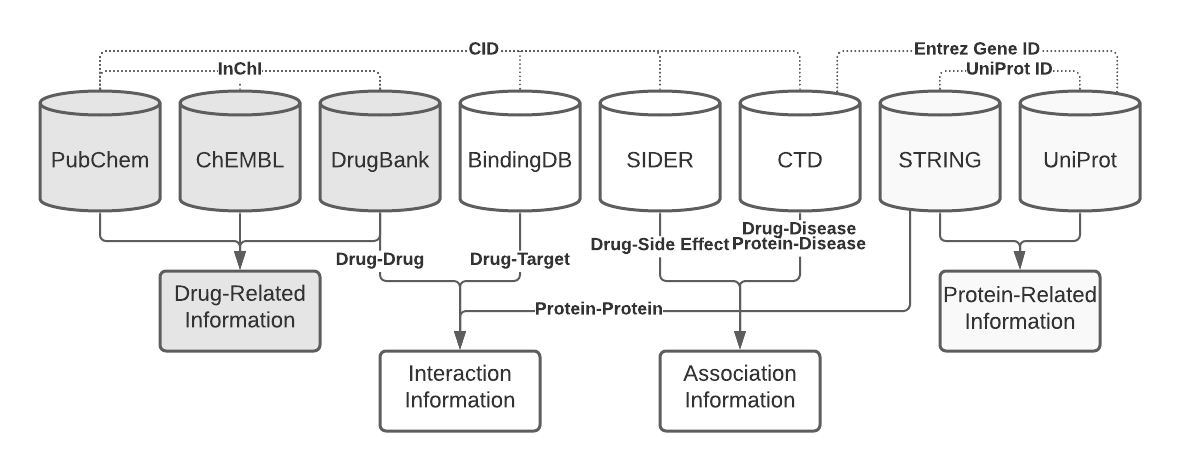
\includegraphics[width=\linewidth]{chapters/materials_and_methods/figures/databases.png}
    \caption{Compiled databases.}
    \label{fig:databases}
\end{figure}

<<<<<<< Updated upstream
=======
<<<<<<< HEAD
\newpage
\subsection{BindingDB}
BindingDB \cite{gilson2016bindingdb} is an online database of drug-target interactions and measured binding affinity values. As of February 2021, BindingDB contains 41,328 entries with DOI, 2,114,159 binding affinity data for 928,022 small molecules, and 8,202 protein targets. Binding affinity is usually expressed in measures such as inhibition constant ($K_i$), dissociation constant ($K_d$), and the half-maximal inhibitory concentration (IC50). For that purpose, 2,077,458 $K_i$ (nM), $K_d$ (nM), and IC50 (nM) values were compiled from the database within the scope of the thesis. 

To benchmark the performance of graph-based representational learning, we use BDB dataset \cite{ozccelik2021chemboost} that is filtered from the BindingDB database. 24,404 binding affinities were observed for all pairs of 924 ligand and 480 proteins, measured by the $pK_d$ value (log-transformed kinase dissociation constant) \cite{ozccelik2021chemboost}. $pK_d$ correlates positively with the binding strength, and the value varies between 1.6 and 13.3. The number of ligands with strong binding affinity values is 3,428 (\textit{i.e.}, $pK_d \geq 7$) according to literature \cite{he2017simboost}. Figure \ref{fig:bdb} illustrates the distribution of the binding affinity values of proteins - ligand pairs in the BDB dataset. 
\begin{figure}
    \centering
        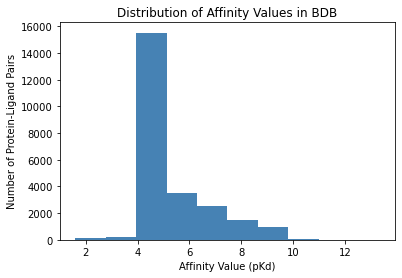
\includegraphics[width=0.5\linewidth]{chapters/materials_and_methods/datasetpreparation/figures/bdb.png} 
    \caption{Distribution of binding affinity values in BDB.}
    \label{fig:bdb}
\end{figure}

%BDB dataset consists of 5 different setups for training and evaluating the model performance. To evaluate the performance of DeepDTA, we trained the DeepDTA model with the knowledge derived from heterogeneous networks on five training setups of BDB dataset \cite{ozccelik2021chemboost}, and tested the models in the corresponding test sets. 
\subsection{ChEMBL}
ChEMBL \cite{davies2015chembl, gaulton2017chembl} is a manually curated chemical database of molecules with drug-like properties and biological activity, which is maintained by the European Molecular Biology Laboratory (EMBL). The ChEMBL database contains bioactivity data of active pharmaceutical ingredients, which are reported with $K_i$, $K_d$, and IC50 values. ChEMBL examines how small molecules interact with target proteins and how these compounds affect cells and whole organisms. Moreover, ChEMBL includes information about the 2D structure, calculated molecular properties, and the ADMET properties such as in vivo absorption, distribution, metabolism, excretion, and toxicity of small molecules. As of May 2020, there are 1,941,412 chemicals in the ChEMBL database and we extract 10,935 drugs' 1D text representations, \textit{i.e.,} SMILES strings from ChEMBL. Using SMILES strings of drugs, we trained the CNN-based model that encodes each SMILES string character as numbers and the language-based model that leverages the similarity between drugs' SMILES strings.
\subsection{Comparative Toxicogenomics Database}
The Comparative Toxicogenomics Database \cite{davis2021comparative} (CTD), is a database that provides information on manually curated chemical–gene$/$protein interactions, chemical-disease, and gene-disease relationships. CTD has several categories of data. These are chemicals, diseases, chemical-disease relationships, and gene-disease relationships. 

\begin{table}[ht]
\caption{CTD statistics (02.2021).}
\vspace{0.25em}
\centering
\begin{tabular}{|l|l|}
\hline
\multicolumn{1}{|c|}{\textbf{Data}} & \multicolumn{1}{c|}{\textbf{Number}} \\ \hline
Chemicals                  & 16,572                      \\ \hline
Diseases                   & 7,246                       \\ \hline
Chemical-Disease Relation  & 2,958,797                   \\ \hline
Gene-Disease Relation      & 28,253,189                  \\ \hline
\end{tabular}
\label{tab:ctd_stats}
\end{table}

Table \ref{tab:ctd_stats} shows the available number of chemicals, diseases, and the association between diseases and chemicals$/$genes, as of February 2021. Since some diseases are common for both chemicals and genes, we extracted 2,958,797 chemical-disease relationships and 28,253,189 gene-disease relationships within the scope of this thesis in order to generate heterogeneous graphs.


\subsection{DrugBank}
DrugBank \cite{wishart2006drugbank, wishart2008drugbank, wishart2018drugbank} is an online database that contains drugs, drug-related data (chemical, pharmacological, and pharmaceutical), and target-related data (sequence, structure, and pathway) as both bioinformatics and cheminformatics sources. As of January 2021, DrugBank contains 14,350 drugs. In the scope of this thesis, we extract 2,682,158 drug-drug interaction information of 14,350 drugs. We create homogeneous and heterogeneous graphs and generate representations for ligands using drugs and the relation between drugs.

% \begin{table}[]
\caption{DrugBank statistics (01.2021).}
\centering
\begin{tabular}{|l|l|}
\hline
\multicolumn{1}{|c|}{\textbf{Data}}  & \multicolumn{1}{c|}{\textbf{Number}} \\ \hline
Total Number of Small Molecule Drugs & 11.834                               \\ \hline
Total Number of Biotech Drugs        & 2.481                                \\ \hline
Total Number of Drugs                & 14.315                               \\ \hline
\end{tabular}
\label{tab:drugbank_stats}
\end{table}

\subsection{PubChem}
PubChem \cite{kim2021pubchem} is an online chemistry database that contains small molecules, nucleotides, as well as information on chemical structures, identifiers, chemical and physical properties. As of February 2021, the current statistics in the database are shown in Table \ref{tab:pubchem_stats}. 

\begin{table}[h]
\caption{PubChem statistics (02.2021)}
\vspace{0.25em}
\centering
\begin{tabular}{|l|l|}
\hline
\multicolumn{1}{|c|}{\textbf{Data}} & \multicolumn{1}{c|}{\textbf{Number}} \\ \hline
Compounds                           & 109,487,163                          \\ \hline
Substances                          & 270,034,522                          \\ \hline
Proteins                            & 96,280                               \\ \hline
Genes                               & 89,655                               \\ \hline
\end{tabular}
\label{tab:pubchem_stats}
\end{table}
\newpage
Since PubChem contains a considerable amount of data, other chemical databases map their entries with PubChem's Compound ID number (CID). In the context of this thesis, we leverage the PubChem CID of each chemical and map with the entries of BindingDB, SIDER, and CTD. Moreover, PubChem contains the International Chemical Identifier (InChI) of chemicals that textually identifies chemical substances. Similar to CID, We used chemicals' InChIs to relate the same chemicals across other databases, ChEMBL and DrugBank, that do not share any common IDs.
\subsection{SIDER}
SIDER \cite{kuhn2010side, kuhn2016sider} is a database of drugs that have entered the market and their recorded adverse drug reactions extracted from public documents and prospectuses. Side effect frequency, drug classification, side effect classification, and drug-target relationships are presented in a computer-readable format. SIDER uses the Anatomical Therapeutic Chemical (ATC) Classification System, a drug classification system that classifies the active substances of drugs according to the organ or system they act on and their therapeutic, pharmacological, and chemical properties. The Medical Dictionary codes side effects for Regulatory Activities (MedDRA) terminology, a clinically validated medical terminology thesaurus. The statistics as of October 2015 are shown in Table \ref{tab:sider_stats}. We used 5,868 side effects and extracted 139,756 drug-side effect relations.
\begin{table}
\caption{SIDER statistics (10.2015).}
\vspace{0.25em}
\centering
\begin{tabular}{|l|l|l|}
\hline
\textbf{Side Effects} & \textbf{Drugs} & \textbf{Drug-Side Effect Pairs} \\ \hline
5,868        & 1,430 & 139,756 \\ \hline
\end{tabular}
\label{tab:sider_stats}
\end{table}

\subsection{STRING}
Search Tool for the Retrieval of Interacting Genes$/$Proteins, STRING \cite{szklarczyk2021string}, is a biological database of known and predicted protein-protein interactions. The interactions include direct (physical) and indirect (functional) associations; they stem from computational prediction, from knowledge transfer between organisms, and interactions aggregated from other (primary) databases.

The STRING database compiles information from several sources such as computational prediction methods, public text collections, laboratory experiments, and other databases. According to the statistics provided as of August 2021, the STRING database contains 67,592,464 proteins and 296,567,750 interactions at the highest security (score $\geq$ 0.900), 834,790,438 interactions with high security or better (score $\geq$ 0.700), medium security or better 3,112,520,562 interactions (score $\geq$ 0.400), and a total of 20,052,394,041 interactions. We leverage the protein-protein interaction data and create a homogeneous database to learn the representations for proteins.
\subsection{UniProt}
The Universal Protein Source (UniProt) \cite{uniprot2021uniprot} is an essential resource for available protein information, including protein sequence and functional information. According to current statistics, as of September 2021, the total number of sequence entries is 565,928. Using amino acid sequences of proteins, we trained the CNN-based model that encodes each amino acid sequence character as numbers and the language-based model that leverages the similarity between proteins' amino acid sequences.


\section{Data Assembling}
\label{section:data_assembling}
This thesis aims to represent chemicals and proteins better. Therefore, chemical and protein-related data from several online databases are compiled. However, this task is not straightforward because of the vast amount of available data and the difficulty of standard mapping information across the databases. Therefore, we analyze the available data in the databases mentioned in Section \ref{section:dataset_compilation} and map the related information using common identifiers or unique sequences. Figure \ref{fig:databases} shows used databases as well as the IDs used to map corresponding databases.

\subsection{Chemical Related Information}
DrugBank, PubChem, and ChEMBL databases are the primary chemical resources, and we mainly focus on them. We compile 14,350 drugs from DrugBank and retrieve their DrugBank IDs and International Chemical Identifiers (InChI) as an initial step. Using InChIs, we connect the data in DrugBank with PubChem and ChEMBL databases and retrieve information about 10,935 different drugs. With 10,935 drugs, we extract 2,196,820 drug-drug relation information from the DrugBank database. Using the PubChem Compound ID number (CID) information available in the PubChem database, we map the PubChem to SIDER and CTD databases. We extract 5,452 distinct side effects from the SIDER database and 115,871 drug-side effect association information for 1,003 drugs. We extract 7,086 distinct diseases from the CTD database and 995,654 drug-disease association information for 3,387 drugs. Finally, we map DrugBank to ChEMBL and compile SMILES representations of 10,935 drugs using the InChI keys. 

Apart from the already existing information, we create a new relation named drug-drug similarity (DDS). Using the compiled SMILES representations of drugs from the ChEMBL database, DDS data is obtained by calculating the similarity of these representations to each other according to the Jaccard Similarity. In order to find similar SMILES sequences, we use the Byte Pair Encoding (BPE) algorithm \cite{sennrich2015neural}. The BPE approach is utilized to identify the language unit vocabulary of chemicals. This method is commonly employed for discovering the tokens of a language in the field of NLP. The BPE algorithm divides SMILES sequences into language units \cite{ozccelik2021debiaseddta}. Then, the similarity of the drugs is calculated in pairs according to the Jaccard Criterion as
\begin{equation}
    Jaccard (A, B) = \frac{|A \cap  B|}{ |A \cup B|} \times  100.
\label{eq:jaccard}
\end{equation}
By calculating the Jaccard Similarities of all drug-drug pairs, we obtain the values shown in Figure \ref{fig:dds}. Accordingly, drug pairs in the dataset with a similarity value greater than $58$ were determined to be similar, with a threshold value determined to cover at least $10\%$ of the whole data, resulting in 2,924,270 drug-drug similarity values for 6,963 distinct drugs.

\begin{figure}[h]
    \centering
        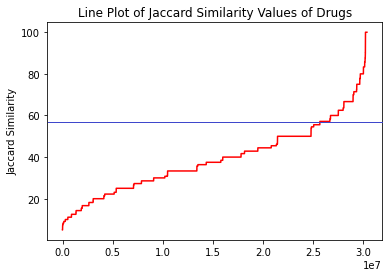
\includegraphics[width=0.5\linewidth]{chapters/materials_and_methods/figures/dds_line.png}
    \caption{Pairwise drug-drug Jaccard similarities.}
    \label{fig:dds}
\end{figure}

\subsection{Protein Related Information}
UniProt and STRING databases are the primary protein resources used in this thesis. We compile 505,250 proteins from the UniProt database, and more specifically, we compile 202,160 proteins belonging to the Homo sapiens and their amino acid sequences. We map 18,876 proteins to the STRING database and extract 183,746 protein-protein interaction information using the UniProt ID from the UniProt database. Finally, using the UniProt ID and Entrez Gene ID, we map the UniProt database to CTD and extract 32,495 protein-disease association information for 32,169 proteins and 126 distinct diseases.

Like the chemicals, in addition to protein-related information, we create a new relation named protein-protein similarity (PPS). Using the compiled amino acid sequences of proteins from the UniProt database, PPS data is obtained by calculating the similarity of these representations to each other according to the Jaccard Similarity of language units found by the BPE algorithm \cite{ozccelik2021debiaseddta}. Then, the similarity of the proteins was calculated in pairs according to the Jaccard Criterion using the formula given in Equation \ref{eq:jaccard}. By calculating the Jaccard Similarities of all protein-protein pairs, we obtained the values shown in Figure \ref{fig:pps}. Accordingly, protein pairs in the dataset with a similarity value greater than $9$ were determined to be similar to each other, with a threshold value was determined to cover at least $11\%$ of the whole data. In the end, we created 528 protein-protein similarity values for 465 distinct proteins.

\begin{figure}[h]
    \centering
        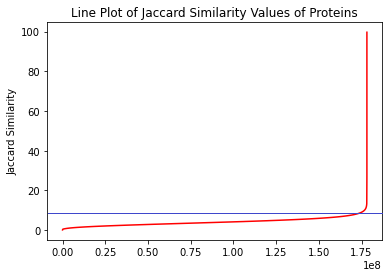
\includegraphics[width=0.5\linewidth]{chapters/materials_and_methods/figures/pps_line.png}
    \caption{Pairwise protein-protein Jaccard similarities.}
=======
>>>>>>> Stashed changes

% TO DO: Which information is used, jaccard vs also, lm
\section{Data Assembling}
\label{section:data_assembling}
Our idea was to represent chemicals and proteins better. Therefore, we compiled chemical and proteins related data from several online databases. And the challenging task was to assemble these compiled large data. For that purpose we analyze the available information in above mentioned databases and and map related information using common data. Figure \ref{fig:databases} shows used databases and the mapping IDs between corresponding databases.

\subsection{Chemical Related Information}
DrugBank, PubChem, and ChEMBL databases are the main resources of chemicals and we mainly focus on them. As an initial step we compile 14.350 drugs from DrugBank and retrieve their DrugBank IDs and InChI (International Chemical Identifier) Keys. Using InChI keys, we map the data in DrugBank to PubChem and ChEMBL databases and able to get the information about 10.935 distinct drugs. With 10.935 drugs, we extract 2.196.820 drug-drug relation information from DrugBank database. Using the PubChem CID (Compound ID number) information available at PubChem database, we map the PubChem to SIDER and CTD databases. From SIDER database, we extract 5452 distinct side effects and 115.871 drug-side effect association information for 1003 drugs. From CTD database, we extract 7086 distinct diseases and 995.654 drug-disease association information for 3387 drugs. Finally, using the InChI keys, we map DrugBank to ChEMBL and compile SMILES (Simplified molecular-input line-entry system) representations of 10.935 drugs. 

Apart from the already existing information we create a new relation, which we named as drug-drug similarity (DDS). Using the compiled SMILES representations of drugs from the ChEMBL (Davies et al., 2015) database, DDS data is obtained by calculating the similarity of these representations to each other according to the Jaccard Similarity Criterion. In order to find the similar SMILES sequences we used the Byte Pair Encoding (BPE) algorithm \cite{sennrich2015neural}. The BPE approach was utilized to identify the language unit vocabulary of chemicals. This method is commonly employed for discovering the tokens of a language, in the field of NLP. The BPE algorithm divided SMILES sequences into language units. Then, the similarity of the drugs was calculated in pairs according to the Jaccard Criterion using the formula given in Equation \ref{eq:jaccard}. By calculating the Jaccard Similarities of all drug-drug pairs, we obtained the values shown in Figure \ref{fig:dds}. Accordingly, drug pairs in the data set with a similarity value greater than $58$ were determined to be similar to each other with a threshold value was determined to cover at least $10\%$ of the whole data. In the end, we created 2.924.270 drug-drug similarity value for 6.963 distinct drugs.

\begin{equation}
    Jaccard (A, B) = \frac{A \cap  B}{ A \cup B} \times  100
\label{eq:jaccard}
\end{equation}

\begin{figure}
    \centering
        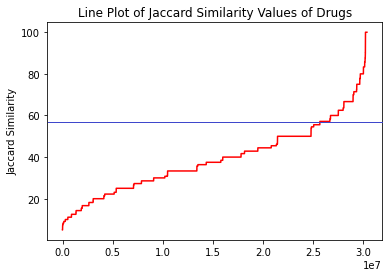
\includegraphics[width=0.5\linewidth]{chapters/materials_and_methods/figures/dds_line.png}
    \caption{Pairwise Drug-Drug Jaccard Similarities.}
    \label{fig:dds}
\end{figure}

%Given a corpus, all uni-characters are first considered as language units by the algorithm. The program then determines the total length of all pairs in the given text. The algorithm, now includes the most common two-character subsequences in the vocabulary. By treating each uni-characters in the vocabulary as a single character, this procedure continues until the goal vocabulary size is generated. The most frequently occurring subsequences of the necessary size are obtained when the method completes.

\subsection{Protein Related Information}
UniProt and STRING databases are main resources used in this thesis. We compile 505.250 proteins from the UniProt database and more specifically we compile 202.160 proteins belonging to the Homo sapiens, as well as their amino acid sequences. Using the UniProt ID from UniProt database, we map 18.876 proteins to STRING database, and extract 183.746 protein-protein interaction information. Finally, using the UniProt ID and Entrez Gene ID we map UniProt database to CTD and extract 32.495 protein-disease association information for 32.169 proteins and 126 distinct diseases.

Similar to the chemicals, besides the already existing protein-related information we create a new relation, which we named as protein-protein similarity (PPS). Using the compiled amino acid  sequences of proteins from the UniProt database, PPS data is obtained by calculating the similarity of these representations to each other according to the Jaccard Similarity Criterion. Again, we employ BPE algorithm to find the language units of protein sequences. Then, the similarity of the proteins was calculated in pairs according to the Jaccard Criterion using the formula given in Equation \ref{eq:jaccard}. By calculating the Jaccard Similarities of all protein-protein pairs, we obtained the values shown in Figure \ref{fig:pps}. Accordingly, protein pairs in the data set with a similarity value greater than $9$ were determined to be similar to each other with a threshold value was determined to cover at least $11\%$ of the whole data. In the end, we created 528 protein-protein similarity value for 465 distinct proteins.


\begin{figure}
    \centering
        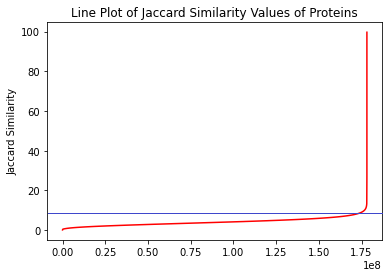
\includegraphics[width=0.5\linewidth]{chapters/materials_and_methods/figures/pps_line.png}
    \caption{Pairwise Protein-Protein Jaccard Similarities.}
<<<<<<< Updated upstream
=======
>>>>>>> d09ebba9e602d1522ef9361417dc21d129009597
>>>>>>> Stashed changes
    \label{fig:pps}
\end{figure}

\section{Graph Creation}
<<<<<<< HEAD
\label{section:graph_generation}
Graphs are used to model complex relations between entities and preserve structural information. In this study, we combine different types of data sources in order to predict binding affinity values between drug-target pairs by using the relevant drug and target-related information. For that purpose, we employ homogeneous and heterogeneous graphs which contain one type of node and relation or many types of nodes and relations, respectively. As discussed in the previous section, we compiled various data, extracted useful information, and then preprocessed them to use with the graph structure. Using PyTorch-Geometric \cite{fey2019fast}, we create graph structures that define node and edge types. Then, we load preprocessed data into graphs and generate positive and negative links between nodes. Observing the relations in the graphs, we sampled the metapaths as mentioned in Section \ref{section:graph_rep_le}. 

% \newpage
\newpage
\begin{table}
\centering
\caption{Homogeneous graph details.}
\vspace{0.25em}
\begin{tabular}{|l|c|c|c|} 
\hline
\multicolumn{1}{|c|}{\begin{tabular}[c]{@{}c@{}}Model\\Name\end{tabular}} & \begin{tabular}[c]{@{}c@{}}Number of\\Nodes\end{tabular} & Metapaths & \begin{tabular}[c]{@{}c@{}}Number of\\Edges\end{tabular} \\ 
\hline
Model (1), (2) & 10935 & Drug Interacts with Drug & 2196820 \\ 
\hline
Model (3), (4) & 6963 & Drug Similar to Drug & 5848540 \\ 
\hline
Model (5), (6) & 12675 & Protein Interacts with Protein & 124536 \\ 
\hline
Model (7), (8) & 465 & Protein Similar to Protein & 1056 \\
\hline
\end{tabular}
\label{tab:homo}
\end{table}

Table \ref{tab:homo} shows details about the Drug-Drug Interaction (DDI), Drug-Drug Similarity (DDS), Protein-Protein Interaction (PPI), and Protein-Protein Similarity (PPS) homogeneous graphs. For DDI relation, we created Model (1) and Model (2) graphs with 10,935 drug nodes and 2,196,820 edges between these nodes. While learning the representation of the graph, we follow the paths from drugs to drugs, so the name of the metapath is ``Drug interacts with the drug." In the case of DDS relation, we created Model (3) and Model (4) graphs with 6,963 drug nodes and 5,848,540 edges between these nodes. While learning the representation of the graph, similarly, we follow the paths from drugs to drugs, so the name of the metapath is ``Drug similar to the drug."


Similarly, we created Model (5) and Model (6) graphs for the PPI relation with 12,675 protein nodes and 124,536 edges between these nodes and the paths from proteins to proteins, with the metapath ``Protein interacts with the protein." Finally, we created Model (7) and Model (8) graphs for the PPS relation with 465 protein nodes and 1056 edges between these nodes, and the paths from proteins to proteins, with the metapath, ``Protein similar to the protein." 

% \newpage
\begin{table}
\centering
\caption{Heterogeneous graphs with disease information.}
\vspace{0.25em}
\begin{tabular}{|l|c|c|c|c|c|} 
\hline
\multicolumn{1}{|c|}{\begin{tabular}[c]{@{}c@{}}Model\\Name\end{tabular}} & \begin{tabular}[c]{@{}c@{}}Num.~of\\Drug\\Nodes\end{tabular} & \begin{tabular}[c]{@{}c@{}}Num. of\\Protein\\Nodes\end{tabular} & \begin{tabular}[c]{@{}c@{}}Num. of\\Disease\\Nodes\end{tabular} & Metapaths & \begin{tabular}[c]{@{}c@{}}Num. of\\Edges\end{tabular} \\ 
\hline
\begin{tabular}[c]{@{}l@{}}Model (9)\\Model (10)\end{tabular} & 3387 & - & 7086 & \begin{tabular}[c]{@{}c@{}}Drug Assoc. with Disease\\Disease Assoc. with Drug\end{tabular} & 1991308 \\ 
\hline
\begin{tabular}[c]{@{}l@{}}Model (11)\\Model (12)\end{tabular} & - & 32169 & 126 & \begin{tabular}[c]{@{}c@{}}Protein Assoc.with Disease\\Disease Assoc.with Protein\end{tabular} & 64990 \\ 
\hline
\begin{tabular}[c]{@{}l@{}}Model (13)\\Model (14)\end{tabular} & 3387 & 32169 & 7087 & \begin{tabular}[c]{@{}c@{}}Drug Assoc. with Disease\\Disease Assoc.with Protein\\Protein Assoc.with Disease\\Disease Assoc.with Drug\end{tabular} & 2056298 \\
\hline
\end{tabular}
\label{tab:het_disease}
\end{table}
Creating heterogeneous graphs needs more effort since the relations between them can be complicated, and the number of information drastically increases the run time. After creating homogeneous graphs, we create heterogeneous graphs using available disease association information. 

\newpage
Table \ref{tab:het_disease} shows details about the Drug-Disease Association (DDiA), Protein-Disease Association (PDiA), and Drug-Disease-Protein Association (DDiPA) heterogeneous graphs. For DDiA relation, we created Model (9) and Model (10) graphs with 3,387 drug nodes, 7,086 disease nodes, and 21,991,308 edges between these nodes. While learning the representation of the graph, we follow the paths from drugs to diseases and vice versa, so the metapaths are ``Drug associates with a disease," and ``Disease reversely associates with a drug." The distinction between the two models is the integration of language models into Model (10) in order to enrich the representation of drugs. Like the DDiA, for the PDiA relation, we created Model (11) and Model (12) graphs with 32,169 protein nodes, 126 disease nodes, and 64,990 edges between these nodes. We follow the paths from proteins to diseases and the reverse paths, so the metapaths are ``Protein associates with a disease," and ``Disease reversely associates with a protein." Similar to Model (10), Model (12) also employs language models. Finally, we combine these two heterogeneous graphs and create one extensive heterogeneous network. Model (13) and Model (14) graphs for the DDiPA relation with 3,387 drug nodes, 6,963 protein nodes, 7087 disease nodes, and 2,056,298 edges between these three nodes. We follow the paths as drug-disease-protein-disease-drug, with the metapaths ``Drug associates with a disease," ``Disease reversely associates with a protein," ``Protein associates with a disease," and ``Disease reversely associates with a drug." To sum up, Model (13) combines the relations between drugs-diseases and proteins-diseases, and Model (14) uses the same types of nodes and relations; however, it integrates language model approaches for biomolecules and diseases to enrich the drug-target representations. 

As an additional experiment, we create another set of models and test the effectiveness of side effect information with these models. Table \ref{tab:het_se} gives details about the Drug-Side Effect Association (DSA) and DDI with DSA heterogeneous graphs. For the DSA graph, we created Model (15) and Model (16) graphs with 1.003 drug nodes, 5,451 side effect nodes, and 231,742 edges between these nodes. While learning the representation of the graph, we follow the paths from drugs to side effects and vice versa, so the metapaths are ``Drug associates with a side effect" and ``Side effect reversely associates with a drug."  DDI is created as in the case of Model (1) and Model (2). For the combination of DDI and DSA graphs, we created Model (17) and Model (18) graphs with 10,932 drug nodes, 5,451 side effect nodes, and 2,427,902 edges between these nodes. We follow the paths from drugs to side effects, side effects to drugs, and drugs to drugs, so the metapaths are ``Drug associates with a side effect," ``Side effect reversely associates with a drug," and ``Drug interacts with a drug." Both Model (16) and Model (18) integrate language models for drugs and side effects.

% \newpage
In order to incorporate language models into the graphs, we used three language model-based representation learning algorithms, namely ProtBERT, ChemBERTa, and BioBERT. 
ProtBERT is a transformer-based model with a masked language modeling objective with 30 layers and 16 attention heads. For each protein sequence, it generates a 1024-length vector as
\begin{equation}
    PB^{t} = \left[\begin{array}{cccccc} pb_1^{t} & pb_2^{t} & pb_3^{t} & \ldots & pb_1014^{t} \end{array} \right].
\end{equation}

\newpage
ProtBERT is based on the BERT model, which is self-supervised and has been pre-trained on a large number of protein sequences. The ProtBERT model is used to initialize the distributional representations of proteins.
=======
% TO DO: Insert node edge numbers, types
% pos and neg edge sampling
\subsection{Homogeneous Graphs}



\subsection{Heterogeneous Graphs}


\section{Learning Distributional Vector Representations}
Machine learning on graph structured data is a ubiquitous task and one of the challenges of this task is to find a way to represent the structure itself and the information it holds so that it can be easily interpreted by mostly used machine learning models. In this thesis, we employ metaPath2Vec \cite{dong2017metapath2vec} model and learn the graph-based distributional representation vectors that reflect the semantic connections in the graph for nodes and edges and finally represent data that cannot be expressed in Euclidean space as a graph.
<<<<<<< Updated upstream
=======
>>>>>>> d09ebba9e602d1522ef9361417dc21d129009597
>>>>>>> Stashed changes

\begin{table}
\centering
\caption{Heterogeneous graphs with side effect information.}
\vspace{0.25em}
\begin{tabular}{|l|c|c|l|c|} 
\hline
\multicolumn{1}{|c|}{\begin{tabular}[c]{@{}c@{}}Model\\Name\end{tabular}} & \begin{tabular}[c]{@{}c@{}}Number\\of~Drug\\Nodes\end{tabular} & \begin{tabular}[c]{@{}c@{}}Number of\\Side~Effect\\Nodes\end{tabular} & \multicolumn{1}{c|}{Metapaths} & \begin{tabular}[c]{@{}c@{}}Number\\of Edges\end{tabular} \\ 
\hline
\begin{tabular}[c]{@{}l@{}}Model (15),\\Model (16)\end{tabular} & 1003 & 5451 & \begin{tabular}[c]{@{}l@{}}Drug Associates with Side Effect\\Side Effect Associates with Drug\end{tabular} & 231742 \\ 
\hline
\begin{tabular}[c]{@{}l@{}}Model (17)\\Model (18)\end{tabular} & 10935 & 5451 & \begin{tabular}[c]{@{}l@{}}Drug Associates with Side Effect\\Side Effect Associates with Drug\\Drug Interacts with Drug\end{tabular} & 2427902 \\
\hline
\end{tabular}
\label{tab:het_se}
\end{table}

To initialize the distributed representations of chemicals, we used the ChemBERTa model pre-trained on 10M PubChem substances using BPE tokenization. ChemBERTa is built on the transformer, has 12 attention heads and six layers, and is pre-trained with masked language modeling.

The BioBERT model was used to initialize the distributed representations of diseases and side effects. Like the previous models, it is a domain-specific language representation model that's been pre-trained on large-scale biological corpora.

<<<<<<< Updated upstream
=======
<<<<<<< HEAD
\section{Learning Distributed Vector Representations}
Representation learning has provided a novel learning paradigm for AI domains. The subject of representation learning is examined and demonstrated in this study, focusing on homogeneous and heterogeneous networks, which contain one type of node and relations or many types of nodes and relations, respectively. The objective of this problem is to automatically project nodes in networks into latent embedding space so that the network's structural and relational properties can be encoded and preserved. Machine learning algorithms can then employ embeddings as features to address relevant downstream machine learning tasks. 
=======
>>>>>>> Stashed changes
% cosine similarity ile val evaluation
% hepsinin sonuclari
>>>>>>> d09ebba9e602d1522ef9361417dc21d129009597

%The majority of heterogeneous network representation learning approaches are inspired by and developed based on homogeneous network representation learning. The primary question is how to encode both the structural and semantic aspects of networks by transforming the structures between different types of nodes and edges into latent spaces. 

Machine learning on graph-structured data is a ubiquitous task, and one of the challenges of this task is to find a way to represent the structure itself and the information it holds so that mainly used machine learning models can easily interpret it. In this thesis, we employ Metapath2Vec \cite{dong2017metapath2vec} model and learn the graph-based distributed representation vectors that reflect the semantic connections in the graph for nodes and edges and finally represent data that cannot be expressed in Euclidean space as a graph.

Metapath2Vec uses priori paths as its basic operating principle, so the paths should be defined in advance, as described in Section \ref{section:graph_rep_le}. Metapath2Vec evaluates different types of edge relations while finding meta paths, that is, paths going from one node to another node, provided that they do not repeat it, and makes semantic inferences using these edges and uses them in vector representations.

ProtBERT and ChemBERTa pre-trained language models are also employed to enrich the distributed vector representations of drugs and proteins learned from the Metapath2Vec algorithm. To do that, we initialize each biomolecule's embeddings with the corresponding vector from pre-trained language models, then start Metapath2Vec's training.

\section{WideDeepDTA}
WideDeepDTA aims to predict binding affinity values of drug-target pairs using information-rich representation vectors of corresponding drugs and targets. In order to generate rich representations, it combines text-based features with network and language model-based representation learning approaches. WideDeepDTA comprises three components, (i) CNN-based DeepDTA model, (ii) graph representation learning, and (iii) affinity prediction.


\subsection{DeepDTA Model}
DeepDTA is an affinity prediction model that uses chemicals' SMILES strings and proteins' amino-acid sequences to represent biomolecules. To represent each character of SMILES and protein sequences, it leverages integer/label encoding with 64 and 25 unique letters, respectively. For instance, the SMILES string ``$ [ C \;\; N \;\;=\;\; C\;\; =\;\; O]$'' is encoded as $[ 1 \;\; 3 \;\; 63\;\; 1 \;\;63\;\; 5]$. Once label encodings are generated, Keras' Embedding Layer is applied to represent characters as 128-dimensional dense vectors. Embeddings are fed into CNN blocks with three 1D-convolutional layers, followed by max-pooling layers. The final feature vectors of SMILES strings and proteins sequences are concatenated and fed into three fully connected neural networks.

\section{Graph Representation Learning}
WideDeepDTA modifies the DeepDTA model and makes it wider. To do that, it combines four input types, namely  SMILES representation and protein sequence representation generated by CNN Blocks; chemical embeddings and protein embeddings generated by graph representation learning. Figure \ref{fig:widerdeepdta} illustrates the overall process. In this section, we explain the details of the WideDeepDTA model.
\begin{figure}
    \centering
        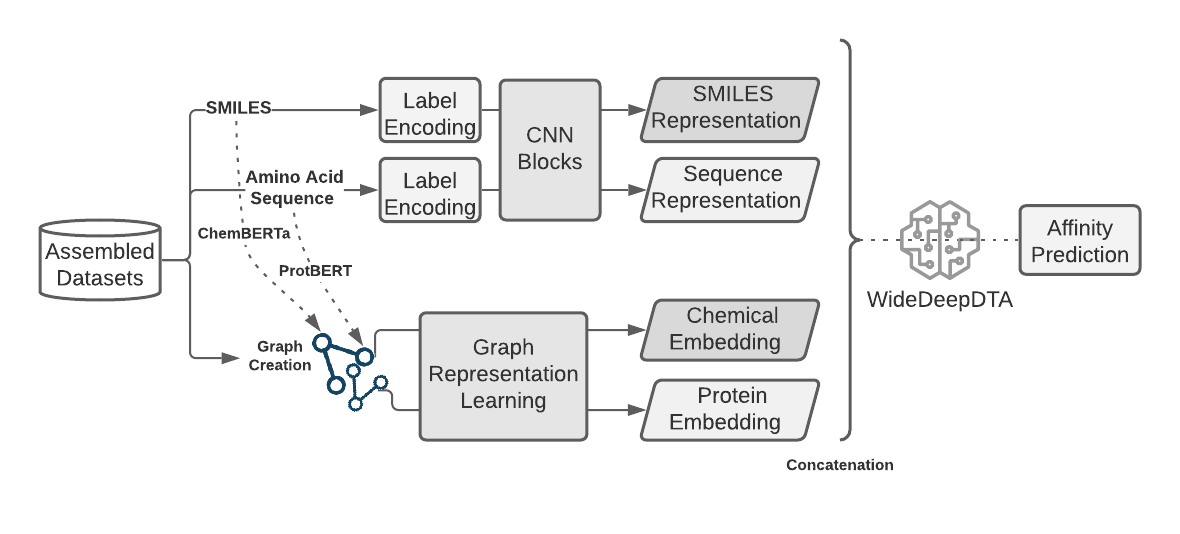
\includegraphics[width=\linewidth]{chapters/materials_and_methods/figures/WiderDeep.png}
    \caption{WideDeepDTA summarized.}
    \label{fig:widerdeepdta}
\end{figure}

After compiling and assembling the datasets, we create our graphs. We define several homogeneous and heterogeneous graphs augmented with the drug and target-related relations explained in Chapter \ref{results}. An example heterogeneous graph is a Drug-Disease-Protein Association (DDiPA) graph. The DDiPA graph $DDiPA(V,\varepsilon))$ consists of a set of drugs $D = {D_1, D_2, …, D_n}$ of $n$ drug nodes, set of targets $T = {P_1, P_2, …, P_m}$ of m protein nodes, and $Di = {Di_1, Di_2, …, Di_t}$ of $t$ disease nodes. DDiPA graph contains two types of edges. The first type of edge represents the association between drug and disease nodes, and the edge from this type is named ``Drug Associates with a Disease." The second type of edge represents the association between protein and disease nodes, and the edge from this type is named ``Protein Associates with a Disease." 

Once the DDiPA graph is created, we load the edges (\textit{i.e.,} positive edges) using drug-disease and protein disease association data extracted from the SIDER database. We split the graph into training and validation sets, in which the validation set contains at least 5\% of the data. Then, we construct the negative samples by generating all possible pairs between drug-disease and protein-disease pairs, then selecting a sample from pairs as many as the number of positive edges in a validation set. Generating negative samples means introducing unknown interactions to the graph to prevent overfitting.

\section{Experimental Setup}
For the whole study, we used Python programming language and performed experiments on Google Colaboratory \cite{carneiro2018performance}, and a machine with NVIDIA Tesla V100 GPU and Intel Xeon Scalable 6148 CPU.

As the training and test folds, we use the same setup in the DeepDTA model. We train each model 5 times with the training set folds, measure the performance on each test set, and report the average results on the BDB dataset. The BDB dataset contains five different training sets and corresponding four different test sets: warm, cold ligand, cold protein, and cold both. The cold ligand test set is used to identify the interactions between unknown ligands and known proteins, \textit{i.e.,} biomolecules that are not used during the training, biomolecules that are used during the training, respectively. The cold protein test set identifies the interactions between known ligands and unknown proteins. Identifying the interactions between known biomolecules form the warm test set, and finally, the interactions between unknown biomolecules form the cold both test set. However, some information related to biomolecules listed as unknown in the test set can be present in the graph creation part. We compute each model's CI, MSE, RMSE, and $R^2$ scores and report the standard deviation in parentheses.

\section{Hyper-parameter Search}
In order to learn distributed representation vectors of chemicals and proteins using the created graphs, we employed the Metapath2Vec model. The Metapath2Vec model uses the train set to train several hyper-parameters such as the embedding size of each embedding vector, walk length throughout the metapath, context size, which is considered for positive samples, and the number of walks to sample for each node in order to find the best model that generated the most convenient representations for the corresponding dataset. The model uses two initialization approaches; (i) random initialization and (ii) initialization using pre-trained language models. In the former case, each node is represented with 32-dimensional vectors initialized as samples from a uniform distribution over $[0,1)$, and in the latter case, each node is represented with 32-dimensional vectors initialized by the pre-trained language models. For that purpose, we used ChemBERTa and ProtBERT pre-trained language models and loaded the embeddings of chemicals and proteins used in the creation of graphs. We also leveraged BioBERT, which is used by the disease names and side effect names associated with the drugs and proteins. In both cases, training goes for 100 epochs, and the model tests the best set of parameters over the validation set. We calculate the training and the validation loss to see the model's performance. 

Since we aim to create better representation for drugs and proteins, we test the success of representations using the cosine similarity metric. Therefore, we first calculate the cosine similarity of positive edges and the cosine similarity of negative edges. Then observe the difference between these two calculations to see whether the model is good at learning the representations or not. In the end, the model sticks with the graph that gives the highest total cosine similarity value. 

Finally, we obtained the low-dimensional representation vectors for each chemical and protein node in the graph. Later on, we concatenate low-dimensional representation vectors of chemicals and proteins generated by the Metapath2Vec algorithm with the representation vectors generated by the CNN blocks. Like the DeepDTA model, combined representation is fed into three fully connected layers. We used 1024 nodes in the first two fully connected layers, followed by a dropout layer of rate $0.1$. The last fully-connected layer contains 512 nodes, followed by the output layer. The proposed model that combines CNN and network-based methods is illustrated in Figure \ref{fig:widedeepdtamodel}.

% \newpage
\section{Affinity Prediction}
Similar to the DeepDTA, the WideDeepDTA model handles the drug-target binding affinity prediction task as a regression problem, using Rectified Linear Unit (ReLU) \cite{nair2010rectified} as the activation function and MSE as the loss function. With MSE, the model aims to maximize the difference between the actual and the predicted value during training. In the case of the CNN-based model, the Adam optimization algorithm \cite{kingma2014adam} is used. In the case of the network-based model
% , the lazy version of the Adam algorithm, namely
SparseAdam is employed. 

\begin{figure}[t]
    \centering
        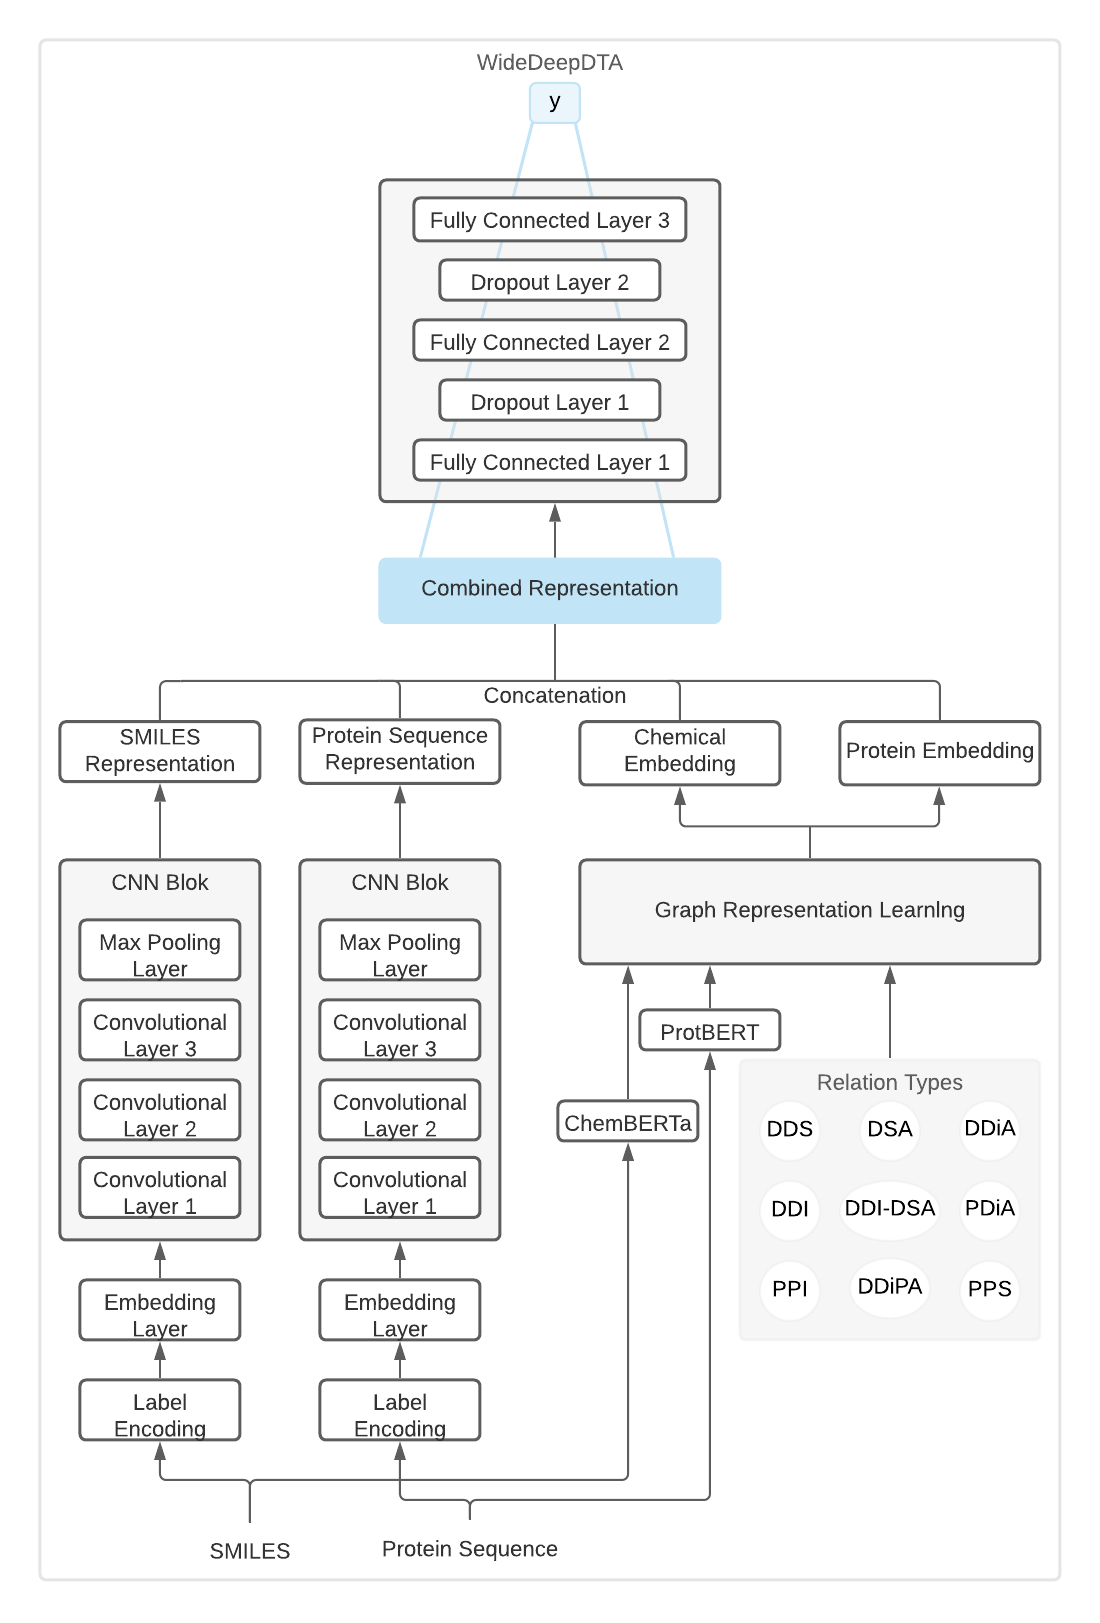
\includegraphics[width=\linewidth]{chapters/materials_and_methods/figures/WiderDeepDTA Model.png}
    \caption{WideDeepDTA in details.}
    \label{fig:widedeepdtamodel}
\end{figure}


<<<<<<< HEAD
% Overall yorumum su: baya guzel bir materyal var burda. Yazdikca yazim kaliten acilmis bence :D Yalniz bu materyal hala biraz daginik. Bence basliklarin yeri degismeli ve sayisi artmali. Basliklarin altindaki bazi materyaller de tam tutmuyor. Re-organize edersen baya duzelecek bence. 
=======
\section{WiderDeepDTA}
In WideDeepDTA, we empowered heterogeneous networks using language models. 
% explain used machines.


\begin{figure}
    \centering
        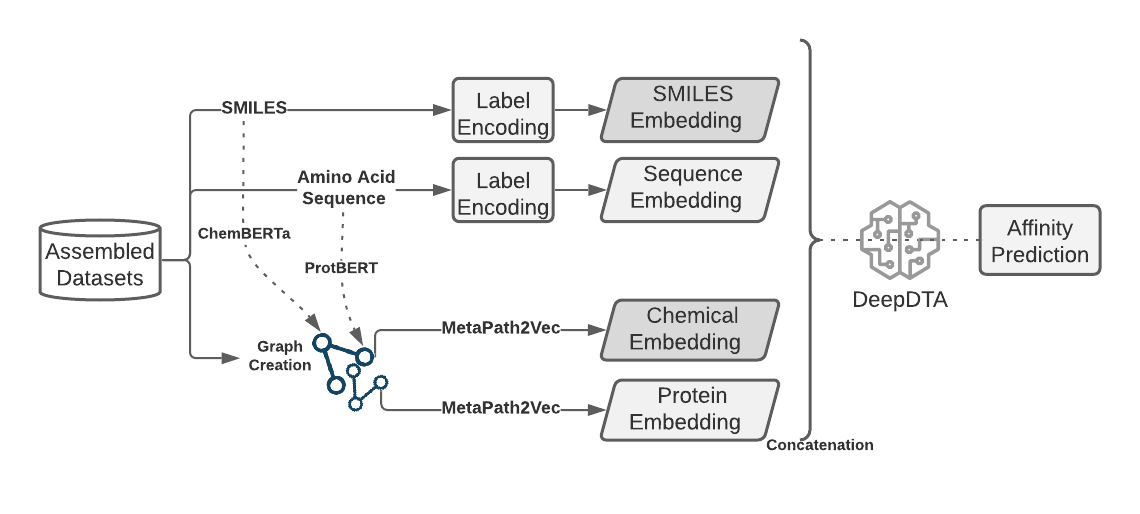
\includegraphics[width=\linewidth]{chapters/materials_and_methods/figures/WiderDeepDTA.png}
    \caption{WideDeepDTA Summarized.}
    \label{fig:widerdeepdta}
\end{figure}


\begin{figure}
    \centering
        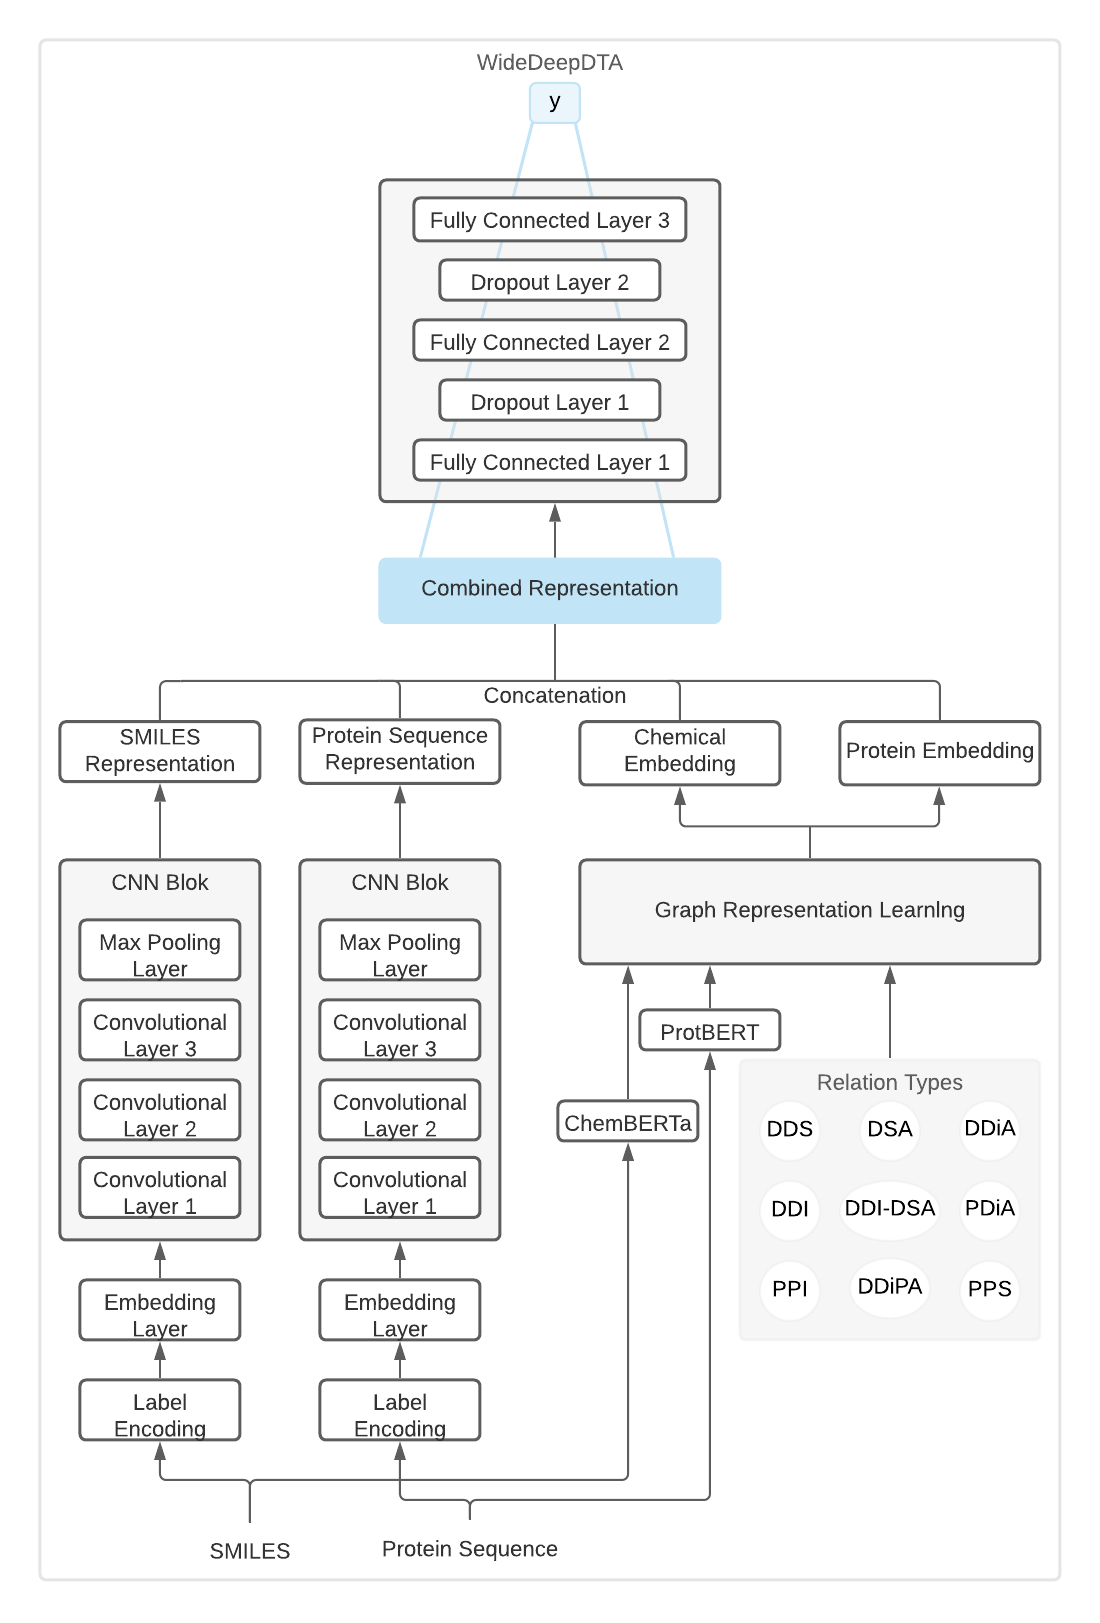
\includegraphics[width=\linewidth]{chapters/materials_and_methods/figures/WiderDeepDTA Model.png}
    \caption{WideDeepDTA in Details.}
    \label{fig:widedeepdtamodel}
<<<<<<< Updated upstream
\end{figure}
=======
\end{figure}
>>>>>>> d09ebba9e602d1522ef9361417dc21d129009597
>>>>>>> Stashed changes
